\documentclass{ctexart}[UTF8]
\usepackage{dirtree}
\usepackage{listings}
\usepackage{xcolor}
\usepackage{graphicx}
\usepackage{enumerate}
\usepackage[a4paper]{geometry} 
\usepackage{amsmath,amsthm,mathtools,amssymb}
\usepackage{mathtools}
\usepackage{diagbox}
\usepackage{multirow,makecell}
\usepackage{float}
\usepackage{url}
\usepackage[nottoc]{tocbibind}
\usepackage{float}
\newcommand{\refe}[1]{Eq.\ref{#1}}
\newcommand{\reft}[1]{Theory.\ref{#1}\ }
\newcommand{\reff}[1]{图\ref{#1}\ }
\lstset{
 columns=fixed,
 numbers=left,                                        % 在左侧显示行号
 numberstyle=\tiny\color{gray},                       % 设定行号格式
 basicstyle=\small\ttfamily,
 frame=none,                                          % 不显示背景边框
 backgroundcolor=\color[RGB]{245,245,244},            % 设定背景颜色
 keywordstyle=\color[RGB]{40,40,255},                 % 设定关键字颜色
 numberstyle=\footnotesize\color{darkgray},           
 commentstyle=\color{gray}\ttfamily,                  % 设置代码注释的格式
 stringstyle=\rmfamily\slshape\color[RGB]{128,0,0},   % 设置字符串格式
 showstringspaces=false,
 breaklines=true,
 language=python
}
\newtheorem{theorem}{Theory}[section]
\geometry{bottom=2cm,left=1cm,right=1cm}
\author{张配天-2018202180}
\title{上机8}
\begin{document}
    \maketitle
    \tableofcontents
    \clearpage
    \section{最长公共子串}
    \subsection{问题描述}
    给定字符串A和字符串B,求解两者包含的有序最长公共子串。
    \subsubsection{输入}
    字符串A和字符串B;
    \subsubsection{输出}
    最长子串及其长度;
    \subsection{算法思路}
    首先分析对于字符串A和B,存在下列情况:\begin{enumerate}
        \item $A[-1] == B[-1]$,此时A和B的LCS由$A[:-1],B[:-1]$的LCS再加上$A[-1]$构成
        \item $A[-1] != B[-1]$,此时分为两种可能\begin{itemize}
            \item A和B的LCS由$A[:-1],B$的LCS构成
            \item A和B的LCS由$A,B[:-1]$的LCS构成
        \end{itemize}
    \end{enumerate}
    \par 于是,我们记$Length[i][j]$为$A[1:i+1]$和$B[1:j+1]$的LCS长度,则有\begin{equation}
        Length[i][j] = \begin{cases}
            0& i=0 or j = 0\\
            Length[i-1][j-1] + 1&A[i] = B[j]\\
            max(Length[i-1][j],length[i][j-1])&A[i]\neq B[j]
        \end{cases}
    \end{equation}
    \subsection{复杂度分析}
    \begin{itemize}
        \item 第17-18行初始化,时间复杂度$\Theta(mn)$
        \item 第22-27行进行三次比较并赋值,可以在$O(6) = O(1)$的时间内完成
        \item 第20-21行循环$(m+1)*(n+1)$词,因此20-27行总时间复杂度$O(mn)$
        \item 第1-10行为重构解的函数,其中每递归一次,$i$和$j$中至少一个元素减一,函数内部进行三次比较,因此时间复杂度$O(3*(m+n)) = O(m+n)$
    \end{itemize}
    \par 综上,整个程序时间复杂度为$\Theta(mn)$,由于优化了重构解的二维数组,因此空间复杂度为$\Theta(mn)$
    \subsection{源代码}
    \begin{lstlisting}
def printLCS(X,Y,length,i,j):
    if i == 0 or j == 0:
        return
    if X[i-1] == Y[j-1] and length[i][j] == length[i-1][j-1]+1:
        printLCS(X,Y,length,i-1,j-1)
        print(X[i-1])
    elif length[i][j] == length[i][j-1]:
        printLCS(X,Y,length,i,j-1)
    elif length[i][j] == length[i-1][j]:
        printLCS(X,Y,length,i-1,j)
        
X = 'ABCBDAB'
Y = 'BDCABA'
m = len(X)
n = len(Y)
length = []
for i in range(m+1):
    length.append([0]*(n+1))

for i in range(1,m+1):
    for j in range(1,n+1):
        if X[i-1] == Y[j-1]:
            length[i][j] = length[i-1][j-1]+1
        elif length[i-1][j] >= length[i][j-1]:
            length[i][j] = length[i-1][j]
        else:
            length[i][j] = length[i][j-1]

print('Length of Longest Common String between %s and %s is %d' % (X,Y,length[m][n]))
print('Longest Common String is: ',end='')
printLCS(X,Y,length,m,n)
    \end{lstlisting}
    \subsection{运行截图}
    \begin{figure}[H]
        \centering
        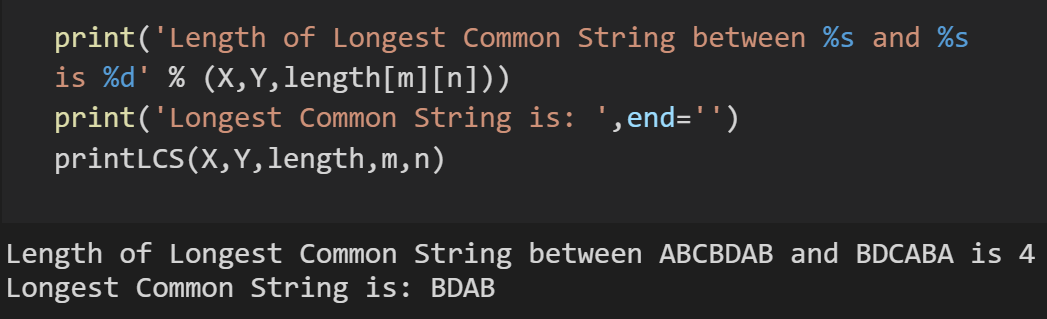
\includegraphics[width=12cm]{resources/8_1.png}
    \end{figure}
    \clearpage
    \section{最优二叉搜索树}
    \subsection{问题描述}
    给定$n$个已经排好序的彼此不同的关键字序列$<k_1,...,k_n>$,访问$k_i$的概率为$p_i$,同时有
    访问$k_j$到$k_j+1$之间的关键字的概率为$q_j(j\in \{0,1,...,n\})$,求解一个二叉搜索树的构造,使得
    整体访问代价期望最小。
    \subsubsection{输入}
    访问$n$个关键字和$n+1$个虚关键字的概率序列$p[n],q[n+1]$
    \subsubsection{输出}
    构造的最优二叉搜索树及访问代价期望。
    \subsection{算法思路}
    和矩阵链乘类似,MatrixChain要求选定一个位置$k$划分括号,将矩阵链分为前半部分和后半部分,
    同时两者必须是最优矩阵链,否则合起来不可能最优;本题考虑将关键字序列划分为根节点前的部分
    和根节点后的部分,两部分各构成子树,子树必须是最优二叉搜索树,否则同理合起来的树不可能最优;
    与矩阵链乘不同的地方在于有了根节点以及存在空子树即$k_{i+1}k_i$的情况,同时虚关键字的存在使得
    关键字子树长度为1时不是平凡的(包含虚关键字),需要在初始化时考虑。\par 
    根据分析,记$Estimate[i][j]$为$k_i,...,k_j$形成的最优二叉搜索树的期望访问代价,则有\begin{equation}
        Estimate[i][j] = \begin{cases}
            q[i-1] & j = i-1\\
            min_{i\leq k\leq j}(Estimate[i][k] + Estimate[k+1][j] + Cost[i][j]) & j \ge i
        \end{cases}
    \end{equation}
    \par 值得注意,这里$i \in \{1,2,...,n+1\}$
    \subsection{复杂度分析}
    \begin{itemize}
        \item 9-18行进行初始化,构建三个二维数组,有时间复杂度$O(n^2 + n) = O(n^2)$
        \item 23-24行计算$j$和$Cost$,可以在$O(2) = O(1)$的时间内完成,重复$O(1+2+\cdots +n) = O(n^2)$次,因此时间复杂度$O(n^2)$
        \item 26-29行计算最小的$tmp$值,也可以在$O(3) = O(1)$的时间内完成,重复$O(n^2 * n) = O(n^3)$次,因此时间复杂度$O(n^3)$
        \item 31-38行重构解,递归输出解,最多需要递归n次,因此在$O(n)$的时间内完成
    \end{itemize}
    \par 综上,总时间复杂度$T(n) = \Theta(n^3)$
    \subsection{源代码}
    \begin{lstlisting}
import math
p = [0,0.15,0.10,0.05,0.10,0.20]
q = [0.05,0.1,0.05,0.05,0.05,0.1]
n = len(p) - 1
Estimate = []
Cost = []
Root = []

for i in range(n+2):
    Estimate.append([math.inf]*(n+1))
    Cost.append([0]*(n+1))
for i in range(n+1):
    Root.append([0]*(n+1))

# 初始化
for i in range(n+1):
    Estimate[i+1][i] = q[i]
    Cost[i+1][i] = q[i]

# l = 1 is not ordinary
for l in range(1,n+1):
    for i in range(1,n-l+2):
        j = i + l
        Cost[i][j-1] = Cost[i][j-2] + p[j-1] + q[j-1]
        for k in range(i,j):
            tmp = Estimate[i][k-1] + Estimate[k+1][j-1] + Cost[i][j-1]
            if tmp < Estimate[i][j-1]:
                Estimate[i][j-1] = tmp
                Root[i][j-1] = k

def printBST(Root,i,j,level):
    if i == j+1:
        return
    else:
        r = Root[i][j]
        print('level:{},key:{}'.format(level,key[r]))
        printBST(Root,i,r-1,level+1)
        printBST(Root,r+1,j,level+1)

print('estimation cost of optimal search binary tree is {}'.format(Estimate[1][n]))
printBST(Root,1,n,0)
\end{lstlisting}
\subsection{运行截图}
\begin{figure}[H]
    \centering
    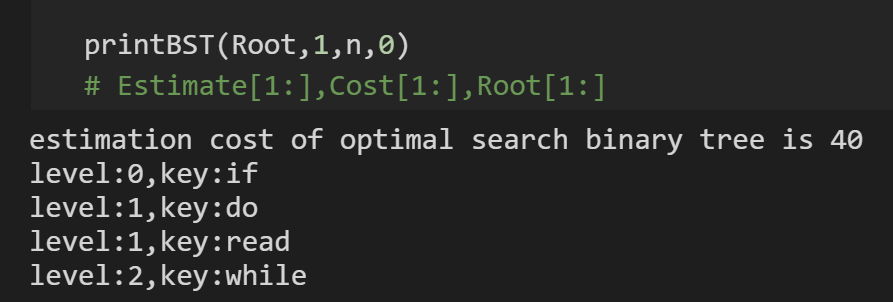
\includegraphics[width=12cm]{resources/8_2.png}
\end{figure}
\end{document}